\section{Stereographic Quantum Signal Processing}
\label{sec:main}

The preceding two sections established the ingredients: a QSP
framework that produces bounded polynomials of a bounded signal
(Section~\ref{sec:preliminaries}), and a stereographic encoding
that places arbitrary complex numbers on the Bloch sphere
(Section~\ref{sec:encoding}).  We now combine them.  The idea is
to feed the stereographically compressed signal
$\rtilde = r/\sqrt{1+r^2} \in [0,1)$ into a standard QSP
circuit, then decode the output by taking the amplitude ratio
$\alpha/\beta$.  Internally, the circuit produces bounded
polynomials $P(\rtilde)$ and $Q(\rtilde)$ satisfying
$|P|^2+|Q|^2=1$; externally, the decoded function
$f(r) = P(\rtilde)/Q(\rtilde)$ is an unbounded rational function
of the original parameter~$r$.  The boundedness constraint is
lifted not by modifying QSP, but by reinterpreting its output
through stereographic decoding.

This section develops the idea in three stages.  First, we define
the stereographic signal operator, show that it reduces to a
rotation for real signals, and derive the Chebyshev states that
arise from repeated application---establishing the base-case
functions of the framework.  Second, we introduce tunable phase
gates to access the full function class, prove that every
achievable function is a rational function of~$r$, and show
that the required QSP phases are obtained by a simple basis
change from the standard protocol.  Third, we analyze the
zero-pole structure and provide an unnormalized formulation
that makes the polynomial arithmetic transparent.  The overall
framework is illustrated in Fig.~\ref{fig:schematic}.

\begin{figure*}[t]
	\centering
	\resizebox{\textwidth}{!}{%
		\begin{tikzpicture}[
				>=Stealth,
				font=\footnotesize,
				every node/.style={inner sep=1pt},
				stage label/.style={font=\footnotesize\bfseries, above},
				arrow label/.style={font=\scriptsize, fill=white, inner sep=1.5pt},
				bounded color/.style={blue!60!black},
				unbounded color/.style={orange!80!red},
			]

			% ============================================================
			%  STAGE 1: ENCODING (left)
			% ============================================================
			\begin{scope}[shift={(0,0)}]
				\node[stage label] at (1.4,2.15) {\textsf{Encoding}};

				% --- Real line (unbounded domain) ---
				\draw[thick, ->] (-0.3,1.2) -- (2.9,1.2)
				node[right, font=\scriptsize] {$r$};
				\foreach \x/\lab in {0.0/0, 0.8/1, 1.6/2, 2.4/3} {
						\draw (\x,1.15) -- (\x,1.25);
						\node[below, font=\tiny] at (\x,1.13) {$\lab$};
					}
				\node[font=\scriptsize, unbounded color] at (1.3,1.55)
				{$r \in [0,\infty)$};
					\draw[thick, densely dotted, unbounded color] (2.6,1.2) -- (2.85,1.2);

					% --- Arrow: stereographic compression ---
					\draw[thick, ->, blue!50!black]
					(1.3,0.95) -- (1.3,0.15)
					node[midway, right, font=\scriptsize, xshift=1pt]
					{$\rtilde = \frac{r}{\sqrt{1{+}r^2}}$};
					\node[font=\tiny, blue!50!black, left] at (0.95,0.55) {SP};

					% --- Bounded interval [0,1) ---
					\draw[thick, ->] (-0.3,-0.15) -- (2.9,-0.15)
					node[right, font=\scriptsize] {$\rtilde$};
					\node[below, font=\tiny] at (0.0,-0.22) {$0$};
					\node[below, font=\tiny] at (2.4,-0.22) {$1$};
					\draw[thick, bounded color, fill=white] (2.4,-0.15) circle (1.5pt);
					\fill[bounded color] (0.0,-0.15) circle (1.5pt);
					\node[font=\scriptsize, bounded color] at (1.3,-0.6)
					{$\rtilde \in [0,1)$ \textnormal{bounded}};

				% --- Bloch sphere (small) ---
				\begin{scope}[shift={(1.3,-1.8)}, scale=0.55]
					\draw[thick] (0,0) circle (1);
					\draw[thick, dashed] (-1,0) arc (180:360:1 and 0.3);
					\draw[thick] (-1,0) arc (180:0:1 and 0.3);
					\fill (0,1) circle (1.5pt) node[above, font=\tiny] {$\ket{0}$};
					\fill (0,-1) circle (1.5pt) node[below, font=\tiny] {$\ket{1}$};
					\draw[thick, ->, blue!60!black] (0,0) -- (0.55,0.65)
					node[right, font=\tiny] {$\ket{r}$};
				\end{scope}
				\node[font=\scriptsize] at (1.3,-2.85)
				{$\ket{r} = \frac{r\ket{0}+\ket{1}}{\sqrt{r^2+1}}$};
			\end{scope}

			% ============================================================
			%  CONNECTING ARROW: Encoding -> QSP
			% ============================================================
			\draw[thick, ->, blue!50!black, shorten >=3pt, shorten <=3pt]
			(3.2,0.0) -- (4.3,0.0)
			node[midway, above, font=\scriptsize] {$\ket{r}$};

			% ============================================================
			%  STAGE 2: QSP CIRCUIT (center)
			% ============================================================
			\begin{scope}[shift={(4.5,0)}]
				\node[stage label] at (2.8,2.15) {\textsf{QSP Circuit}};

				% Wire
				\draw[thick] (0.0,0.0) -- (5.6,0.0);
				\node[left, font=\scriptsize] at (-0.05,0.0) {$\ket{0}$};

				% Phase gates (blue) and signal operators (orange)
				\node[draw, fill=blue!8, minimum width=0.55cm, minimum height=0.5cm,
					font=\scriptsize] (phid) at (0.45,0.0) {$\phi_d$};
				\node[draw, fill=orange!15, minimum width=0.55cm, minimum height=0.5cm,
					font=\scriptsize] (sz1) at (1.2,0.0) {$S_z$};
				\node[draw, fill=blue!8, minimum width=0.55cm, minimum height=0.5cm,
					font=\scriptsize] (phid1) at (1.95,0.0) {$\phi_{d\text{-}1}$};
				\node[font=\normalsize] at (2.65,0.0) {$\cdots$};
				\node[draw, fill=orange!15, minimum width=0.55cm, minimum height=0.5cm,
					font=\scriptsize] (sz2) at (3.35,0.0) {$S_z$};
				\node[draw, fill=blue!8, minimum width=0.55cm, minimum height=0.5cm,
					font=\scriptsize] (phi1) at (4.1,0.0) {$\phi_1$};
				\node[draw, fill=orange!15, minimum width=0.55cm, minimum height=0.5cm,
					font=\scriptsize] (sz3) at (4.85,0.0) {$S_z$};
				\node[draw, fill=blue!8, minimum width=0.55cm, minimum height=0.5cm,
					font=\scriptsize] (phi0) at (5.6,0.0) {$\phi_0$};

				% Output state
				\node[right, font=\scriptsize] at (5.95,0.0)
				{$P\ket{0}{+}Q\ket{1}$};

				% Brace: unitarity constraint
				\draw[decorate, decoration={brace, amplitude=4pt, mirror}]
				(0.1,-0.50) -- (5.95,-0.50)
				node[midway, below=5pt, font=\scriptsize, bounded color]
				{$|P(\rtilde)|^2 + |Q(\rtilde)|^2 = 1$
					\quad $\Rightarrow$ \quad $|P|,|Q| \leq 1$ \textnormal{bounded}};

				% Basis change identity
				\node[font=\scriptsize, text=gray] at (2.8,0.75)
				{$S_z = V^{-1} W(\rtilde)\, V$, \quad $V = \mathrm{diag}(1,i)$};
				\node[font=\scriptsize, text=gray] at (2.8,1.2)
				{degree $d$ \quad ($d+1$ phases, $d$ signal operators)};

				% Block-encoding context
				\node[font=\scriptsize, text=gray!70!black, align=center] at (2.8,-1.6)
				{In block-encoding context:\\[1pt]
					ancilla hosts QSP;
					system register selects $\lambda_j$};

				% Small block encoding circuit
				\begin{scope}[shift={(0.7,-2.55)}, scale=0.8]
					\draw[thick] (0,0.6) -- (4.2,0.6);
					\node[left, font=\tiny] at (0,0.6) {$\ket{0}_a$};
					\draw[thick] (0,0) -- (4.2,0);
					\node[left, font=\tiny] at (0,0) {$\ket{\psi}_s$};
					\node[draw, fill=green!8, minimum width=0.5cm, minimum height=0.8cm,
						font=\tiny] at (0.6,0) {$V$};
					\node[draw, fill=orange!12, minimum width=1.2cm, minimum height=0.4cm,
						font=\tiny] at (2.1,0.6) {\textsf{QSP}$(\bm\phi)$};
					\draw[thick] (2.1,0.38) -- (2.1,0.08);
					\fill (2.1,0.0) circle (1.5pt);
					\node[draw, fill=green!8, minimum width=0.5cm, minimum height=0.8cm,
						font=\tiny] at (3.6,0) {$V^\dagger$};
					\node[draw, fill=gray!10, minimum width=0.35cm, minimum height=0.35cm,
						font=\tiny] at (4.0,0.6) {$M$};
				\end{scope}
			\end{scope}

			% ============================================================
			%  CONNECTING ARROW: QSP -> Decoding
			% ============================================================
			\draw[thick, ->, orange!70!red, shorten >=3pt, shorten <=3pt]
			(11.2,0.0) -- (12.3,0.0);
			\node[font=\scriptsize, orange!70!red, above] at (11.75,0.35)
			{$\langle\PauliZ\rangle$};
			\node[font=\scriptsize, orange!70!red, below] at (11.75,-0.35)
			{$\langle\PauliX\rangle$};

			% ============================================================
			%  STAGE 3: DECODING (right)
			% ============================================================
			\begin{scope}[shift={(12.5,0)}]
				\node[stage label] at (1.6,2.15) {\textsf{Decoding}};

				% Decoding formula
				\node[font=\scriptsize, align=center] at (1.6,1.45)
				{Pauli measurement\\[2pt]
					$f(r) = \dfrac{P(\rtilde)}{Q(\rtilde)}$};

				% Key insight box
				\node[draw, rounded corners=3pt, fill=orange!8,
					font=\scriptsize, align=center,
					minimum width=2.8cm, inner sep=4pt]
				at (1.6,0.25)
				{$|P|,|Q| \leq 1$ \textit{bounded}\\[3pt]
					but $P/Q$ can \textbf{diverge}\\[2pt]
					where $Q(\rtilde) = 0$};

				% Small plot: bounded |P| vs unbounded P/Q
				\begin{scope}[shift={(0.15,-2.3)}, xscale=0.35, yscale=0.14]
					\draw[->, thin] (-0.3,0) -- (8.8,0) node[right, font=\tiny] {$r$};
					\draw[->, thin] (0,-7.5) -- (0,8) node[above, font=\tiny] {};
					\draw[thin, dashed, gray!60] (-0.2,5) -- (8.5,5);
					\draw[thin, dashed, gray!60] (-0.2,-5) -- (8.5,-5);
					\node[font=\tiny, gray, left] at (-0.2,5) {$1$};
					\node[font=\tiny, gray, left] at (-0.2,-5) {$\text{-}1$};
					\fill[blue!5] (-0.2,-5) rectangle (8.5,5);

					% |P| bounded curve
					\draw[very thick, bounded color, domain=0.2:8.5, samples=60, smooth]
					plot (\x, {5*sin(deg(1.8*\x))*exp(-0.12*\x)});
					\node[font=\tiny, bounded color] at (6.8,2.5) {$|P(\rtilde)|$};

					% P/Q unbounded curve with pole
					\draw[very thick, unbounded color, domain=0.2:0.92, samples=25, smooth]
					plot (\x, {min(7.5, 1.5*\x/(\x - 1.0))});
					\draw[very thick, unbounded color, domain=1.1:8.5, samples=40, smooth]
					plot (\x, {max(-7.5, 1.5*\x/(\x - 1.0))});

					% Pole line
					\draw[thin, densely dotted, red!60!black] (1.0,-7.5) -- (1.0,7.5);
					\node[font=\tiny, red!60!black, above] at (1.0,7.5) {\tiny pole};

					\node[font=\tiny, unbounded color] at (5.5,-6.5) {$P/Q$ \textbf{unbounded}};
				\end{scope}

				% Output domain
				\node[font=\scriptsize, unbounded color] at (1.6,-3.7)
				{$f(r) \in (-\infty, +\infty)$};
			\end{scope}

			% ============================================================
			%  OVERALL FLOW ARROW (top)
			% ============================================================
			\draw[thick, ->, gray!40, line width=1.2pt,
				shorten >=5pt, shorten <=5pt]
			(0.5,2.5) to[out=20, in=160] (14.5,2.5);
			\node[font=\scriptsize, gray!50, above] at (7.5,3.0)
			{$r \in [0,\infty) \;\;\longrightarrow\;\;
			f(r) \in (-\infty,+\infty)$: unbounded input $\to$ unbounded output};

		\end{tikzpicture}%
	}% end resizebox
	\caption{Schematic of the stereographic QSP framework, showing the three stages that lift the boundedness constraint. \textit{Left (Encoding):} An unbounded parameter $r \in [0,\infty)$ is compressed into the bounded QSP domain $\rtilde = r/\sqrt{1+r^2} \in [0,1)$ via stereographic projection~(SP), producing the single-qubit state $\ket{r}$ on the Bloch sphere. \textit{Center (QSP Circuit):} The standard QSP sequence of alternating phase gates $\exp[i\phi_k\PauliZ]$ and stereographic signal operators $S_z$ acts on $\ket{0}$, producing the output state $P(\rtilde)\ket{0} + Q(\rtilde)\ket{1}$ with $|P|^2+|Q|^2=1$. The stereographic and standard signal operators are related by $S_z = V^{-1}W(\rtilde)V$ with $V = \mathrm{diag}(1,i)$, so all existing QSP machinery applies directly. The lower inset shows the block-encoding context for multi-qubit operators. \textit{Right (Decoding):} Pauli measurements on the output state yield the ratio $f(r) = P(\rtilde)/Q(\rtilde)$, which diverges wherever $Q(\rtilde) = 0$. The inset plot illustrates the central mechanism: the internal polynomial $|P(\rtilde)|$ (blue) remains bounded within $[-1,1]$, but the decoded ratio $P/Q$ (orange) is an unbounded rational function with poles. The unitarity constraint does not imply bounded output.}
	\label{fig:schematic}
\end{figure*}

\subsection{Signal Operator and Chebyshev States}
\label{subsec:signal-chebyshev}

Every QSP protocol requires a signal unitary---the gate that
encodes the parameter to be processed.  In the standard
framework this is $W(a)$, whose diagonal entry is the bounded
signal $a \in [-1,1]$.  For stereographic QSP the analogous
object must encode an \emph{unbounded} parameter~$r$ into a
unitary gate.  The natural choice is to compose the encoding
unitary $U_z$ from~\eqref{eq:encoding-unitary} with
a Pauli gate that flips the second column, producing a unitary
whose matrix elements depend on~$r$ through the compressed
variable $\rtilde = r/\sqrt{1+r^2}$.

\begin{definition}[Signal Operator]
	\label{def:signal-operator}
	For $z = re^{i\theta}$, the stereographic signal operator is
	\begin{equation}
		S_z \equiv U_z\,\PauliZ,
		\label{eq:signal-operator}
	\end{equation}
	where $U_z$ is the encoding unitary~\eqref{eq:encoding-unitary}.
\end{definition}

Multiplying out, the columns of $U_z$ are swapped and
sign-flipped by $\PauliZ$, so $S_z$ has diagonal entries
$re^{\pm i\theta}/\sqrt{1+r^2}$ and off-diagonal entries
$\mp 1/\sqrt{1+r^2}$.  Comparing with the standard signal
unitary $W(a)$ from~\eqref{eq:standard-signal}, the diagonal
entries play the same role---they carry the signal---but the
off-diagonal elements differ: $\pm 1/\sqrt{1+r^2}$ instead of
$\pm i\sqrt{1-a^2}$.  This difference is a phase ($i$ versus
$1$) that will be absorbed by a basis change in
Section~\ref{subsec:qsp-phases}.  For now, the important
observation is that $S_z$ is unitary for every $r \geq 0$,
including $r \to \infty$ where $S_z \to \PauliZ$, so no
truncation or rescaling of the signal is ever needed.

The structure of $S_z$ becomes especially transparent for real
signals ($\theta = 0$), which is the case relevant to
Hermitian eigenvalues.  Setting $\theta = 0$ and identifying
$\cos\phi = r/\sqrt{1+r^2}$, $\sin\phi = 1/\sqrt{1+r^2}$,
the signal operator reduces to a rotation:
\begin{equation}
	S_z\big|_{\theta=0} = \begin{pmatrix} \cos\phi & -\sin\phi \\ \sin\phi & \cos\phi \end{pmatrix} \equiv R(\phi),
	\label{eq:rotation-form}
\end{equation}
where $\phi = \arccos(\rtilde)$ and $\rtilde = r/\sqrt{1+r^2}$.

Since $R(\phi)$ is a rotation, its $k$-th power is
$R(k\phi)$---and the entries of a rotation matrix evaluated at
a multiple angle are precisely Chebyshev polynomials (recall
Section~\ref{sec:preliminaries}).

\begin{theorem}[Chebyshev States]
	\label{thm:chebyshev}
	The $k$-fold signal operator applied to $\ket{0}$ produces
	\begin{equation}
		S_z^k\ket{0} = T_k(\rtilde)\,\ket{0} + \frac{U_{k-1}(\rtilde)}{\sqrt{1+r^2}}\,\ket{1},
		\label{eq:chebyshev-state}
	\end{equation}
	where $T_k$ and $U_{k-1}$ are Chebyshev polynomials of the first and second kind evaluated at $\rtilde = r/\sqrt{1+r^2}$.
\end{theorem}

The proof is a direct application of the Chebyshev identities
to the rotation~\eqref{eq:rotation-form}; see
Appendix~\ref{app:proofs}.

The Chebyshev states~\eqref{eq:chebyshev-state} are the
base-case outputs of stereographic QSP: each is fully
determined by the signal~$r$, with no tunable phases.
Internally, the $\ket{0}$-amplitude $T_k(\rtilde)$ is a
bounded polynomial satisfying $|T_k(\rtilde)| \leq 1$, just
as in standard QSP.  The question is what happens when we
\emph{decode}---that is, when we apply the stereographic
decoding formula~\eqref{eq:decoding} to read out the encoded value.
Since decoding takes a ratio of amplitudes, the normalization
constraint $|T_k|^2 + |U_{k-1}/\sqrt{1+r^2}|^2 = 1$ no
longer implies a bounded output: the ratio can diverge wherever
the denominator vanishes.

\begin{theorem}[Unbounded Rational Functions]
	\label{thm:unbounded}
	Decoding the $k$-fold signal state~\eqref{eq:chebyshev-state} produces the unbounded rational function
	\begin{equation}
		z_k(r) = \frac{T_k(\rtilde)\,\sqrt{1+r^2}}{U_{k-1}(\rtilde)} = \cot\!\big(k\arctan(1/r)\big).
		\label{eq:cot-identity}
	\end{equation}
\end{theorem}

\begin{proof}
	The state~\eqref{eq:chebyshev-state} has the form $\alpha\ket{0} + \beta\ket{1}$ with $\alpha = T_k(\rtilde)$ and $\beta = U_{k-1}(\rtilde)/\sqrt{1+r^2}$. The decoded value is
	\begin{equation}
		z_k = \frac{\alpha}{\beta} = \frac{T_k(\rtilde)\sqrt{1+r^2}}{U_{k-1}(\rtilde)}.
	\end{equation}
	Setting $\phi = \arctan(1/r)$, so that $\cos\phi = r/\sqrt{1+r^2} = \rtilde$ and $\sin\phi = 1/\sqrt{1+r^2}$, the Chebyshev definitions give $T_k(\rtilde) = \cos(k\phi)$ and $U_{k-1}(\rtilde)\sin\phi = \sin(k\phi)$. Substituting:
	\begin{equation}
		z_k = \frac{\cos(k\phi)\sqrt{1+r^2}}{U_{k-1}(\rtilde)} = \frac{\cos(k\phi)}{\sin(k\phi)} = \cot(k\phi),
	\end{equation}
	where the second equality uses $U_{k-1}(\rtilde) = \sin(k\phi)/\sin\phi = \sin(k\phi)\sqrt{1+r^2}$.
\end{proof}

Theorem~\ref{thm:unbounded} is the central result of this
paper.  The decoded function $\cot(k\arctan(1/r))$ is
unbounded---it diverges at each of its $k-1$ poles on
$(0,\infty)$---yet it is produced by a unitary circuit whose
internal amplitudes never exceed~$1$.  The boundedness
constraint is not violated; it is \emph{circumvented} by the
decoding step, which extracts a ratio rather than an amplitude.
In standard QSP the output is the amplitude $T_k(a)$ itself,
bounded by construction.  Here the output is the ratio
$T_k(\rtilde)/[U_{k-1}(\rtilde)/\sqrt{1+r^2}]$, and the
unitarity condition $|P|^2+|Q|^2=1$ guarantees only that the
numerator and denominator cannot both vanish---not that their
ratio is bounded.

Beyond its role as a base case, the Chebyshev
state~\eqref{eq:chebyshev-state} connects stereographic QSP
to a well-studied family of orthogonal functions on the real
line.  The components of $S_z^k\ket{0}$, when viewed as
functions of~$r$ rather than~$\rtilde$, are precisely the
\emph{rational Chebyshev functions} introduced by
Boyd~\cite{Boyd1990,Boyd1987}:
\label{subsec:rational-chebyshev}
\begin{align}
	\TB_k(r) & \equiv T_k\!\!\left(\frac{r}{\sqrt{1+r^2}}\right), \nonumber                \\
	\SB_k(r) & \equiv \frac{U_{k-1}\!\!\left(\frac{r}{\sqrt{1+r^2}}\right)}{\sqrt{1+r^2}}.
	\label{eq:rational-chebyshev}
\end{align}
These are obtained from the standard Chebyshev polynomials by
the algebraic change of variable
$t = r/\sqrt{1+r^2}$, which maps
$(-\infty, \infty) \to (-1,1)$.  In this notation the
Chebyshev state takes the compact form
\begin{equation}
	S_z^k\ket{0} = \TB_k(r)\,\ket{0} + \SB_k(r)\,\ket{1}.
	\label{eq:rational-chebyshev-state}
\end{equation}

The connection to Boyd's work is not merely notational.  The
rational Chebyshev functions satisfy the orthogonality
relation
\begin{equation}
	\int_{-\infty}^{\infty} \TB_j(r)\,\TB_k(r)\,\frac{dr}{1+r^2} = c_k\,\delta_{jk},
	\label{eq:orthogonality}
\end{equation}
where $c_0 = \pi$ and $c_k = \pi/2$ for $k \geq 1$, and
similarly for $\SB_k$.  This follows from the standard
Chebyshev orthogonality after the substitution
$t = r/\sqrt{1+r^2}$, which transforms the measure as
$dt/\sqrt{1-t^2} = dr/(1+r^2)$.  The resulting weight
function $1/(1+r^2)$ is the Cauchy--Lorentz distribution, and
the rational Chebyshev basis provides spectrally convergent
expansions for functions on the real line that decay
algebraically at infinity~\cite{Boyd1987}.  The approximation
theory developed by Boyd for functions on unbounded
domains~\cite{Boyd1990} therefore applies directly to
stereographic QSP, providing rigorous convergence guarantees
for polynomial approximations in the $\rtilde$ variable.
The first several rational Chebyshev functions and the
corresponding decoded functions
$z_k(r) = \TB_k(r)/\SB_k(r) = \cot(k\arctan(1/r))$ are
plotted in Fig.~\ref{fig:rational-chebyshev}.

\begin{figure*}[t]
	\centering
	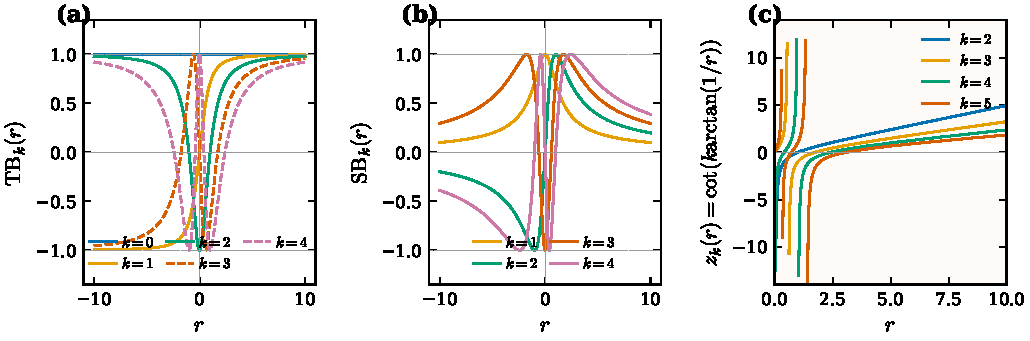
\includegraphics[width=\textwidth]{figures/rational_chebyshev.pdf}
	\caption{Stereographic QSP operates on unbounded rational functions built from bounded basis elements. (a)~Rational Chebyshev functions $\TB_k(r) = T_k(r/\sqrt{1+r^2})$ for $k=0,\ldots,4$: these are standard Chebyshev polynomials composed with the stereographic compression $r \mapsto r/\sqrt{1+r^2}$, and remain bounded by $1$ on the entire real line. (b)~The complementary basis functions $\SB_k(r) = U_{k-1}(r/\sqrt{1+r^2})/\sqrt{1+r^2}$, also bounded. Together, $\TB_k$ and $\SB_k$ form the components of the Chebyshev state $S_z^k\ket{0}$. (c)~Decoded cotangent functions $z_k(r) = \TB_k(r)/\SB_k(r) = \cot(k\arctan(1/r))$. Despite being ratios of bounded functions, these are \emph{unbounded} rational functions of $r$ with $k$ interlacing zeros and poles (red shading indicates the region $|z_k| > 1$ inaccessible to standard QSP). This illustrates the central mechanism: stereographic decoding converts bounded QSP outputs into unbounded rational functions.}
	\label{fig:rational-chebyshev}
\end{figure*}

\subsection{Full Protocol and Reduction to Standard QSP}
\label{subsec:qsp-phases}

The base-case functions
$z_k(r) = \cot(k\arctan(1/r))$ demonstrate the central
mechanism---decoding converts bounded Chebyshev states into
unbounded rational functions---but they form only a
one-parameter family, indexed by the iteration count~$k$, with
no tunability beyond the choice of degree.  For applications one
needs \emph{arbitrary} rational transformations of the signal.
Just as in standard QSP, where tunable phase gates between
signal applications unlock the full polynomial class
(Section~\ref{sec:preliminaries}), the same strategy applies
to the stereographic signal operator.
A degree-$d$ stereographic QSP sequence with phases
$\bm{\phi} = (\phi_0, \ldots, \phi_d)$ alternates $d$ signal
operators with $d+1$ phase rotations:
\begin{equation}
	W_{\bm{\phi}}(r) = \exp[i\phi_0\PauliZ]\,S_z\, \exp[i\phi_1\PauliZ]\,S_z \cdots S_z\, \exp[i\phi_d\PauliZ],
	\label{eq:stereo-qsp}
\end{equation}
with the corresponding circuit:
\begin{equation}
	\begin{quantikz}[column sep=0.25cm, row sep=0.3cm]
		\lstick{\footnotesize$\ket{0}$} & \gate{\phi_d} & \gate{S_z} & \gate{\phi_{d\text{-}1}} & \ \cdots\ \qw & \gate{S_z} & \gate{\phi_0} & \qw
	\end{quantikz}
	\label{eq:qsp-circuit}
\end{equation}
where each $\phi_j$ box denotes the phase gate
$R_z(\phi_j) \equiv \exp[i\phi_j\PauliZ]$ and $S_z$ is the
stereographic signal
operator~\eqref{eq:signal-operator}.  The structure is
identical to~\eqref{eq:standard-qsp}---the same alternation
of signal and phase operations---with $S_z$ replacing $W(a)$.

This structural parallel is not a coincidence.  The comparison
after Definition~\ref{def:signal-operator} showed that $S_z$
and $W(a)$ have the same diagonal entries but differ in the
phase of their off-diagonal elements: $\pm 1/\sqrt{1+r^2}$
versus $\pm i\sqrt{1-a^2}$.  When $a = \rtilde$, these
off-diagonal entries have the same magnitude
($1/\sqrt{1+r^2} = \sqrt{1-\rtilde^2}$) and differ only by a
factor of~$i$.  A factor of~$i$ in the off-diagonal of an
$\SU(2)$ matrix is precisely what conjugation by a diagonal
phase matrix can produce.  This observation suggests that the
two signal operators are related by a fixed change of basis,
and that the entire stereographic protocol reduces to standard
QSP after this change of basis.  The following proposition
confirms it.

\begin{proposition}[Basis Change]
	\label{prop:basis-change}
	Let $V$ be the diagonal unitary with entries $(1,0;\,0,i)$.  The stereographic signal operator~\eqref{eq:signal-operator} and the standard signal unitary~\eqref{eq:standard-signal} are related by $S_z = V^{-1}\,W(\rtilde)\,V$ with $\rtilde = r/\sqrt{1+r^2}$, and the phase operator is invariant under conjugation: $V^{-1}\exp[i\phi\PauliZ]\,V = \exp[i\phi\PauliZ]$.  Consequently, writing $W_{\bm{\phi}}^{\mathrm{(stereo)}}(r)$ for the stereographic QSP product~\eqref{eq:stereo-qsp} and $U_{\bm{\phi}}^{\mathrm{(std)}}(\rtilde)$ for the standard QSP product~\eqref{eq:standard-qsp} evaluated at $a = \rtilde$,
	\begin{equation}
		W_{\bm{\phi}}^{\mathrm{(stereo)}}(r) = V^{-1}\,U_{\bm{\phi}}^{\mathrm{(std)}}(\rtilde)\,V.
		\label{eq:basis-change}
	\end{equation}
\end{proposition}

\begin{proof}
	For part (1), direct computation gives
	\begin{equation}
		V^{-1}W(\rtilde)V = \begin{pmatrix} \rtilde & -\sqrt{1-\rtilde^2} \\ \sqrt{1-\rtilde^2} & \rtilde\end{pmatrix} = S_z\big|_{\theta=0}, \nonumber
	\end{equation}
	since $\sqrt{1-\rtilde^2} = 1/\sqrt{1+r^2}$. Part~(2) is
	immediate: $\exp[i\phi\PauliZ] = \mathrm{diag}(e^{i\phi},
		e^{-i\phi})$ commutes with $V = \mathrm{diag}(1, i)$, since
	both are diagonal.
	Equation~\eqref{eq:basis-change} then follows by
	telescoping the product~\eqref{eq:stereo-qsp}: every
	$S_z = V^{-1}WV$ contributes a pair of $V$ factors, and
	the invariance of the phase gates ensures that all
	intermediate $VV^{-1}$ pairs cancel, leaving a single
	$V^{-1}$ on the left and $V$ on the right.
\end{proof}

The content of Equation~\eqref{eq:basis-change} is that every
stereographic QSP circuit is a standard QSP circuit in
disguise, conjugated by a fixed gate~$V$ that depends on
neither the signal nor the phases.  This has two immediate
consequences.

First, conjugation by the diagonal matrix~$V$ does not alter
diagonal matrix elements, so
$\bra{0}W_{\bm{\phi}}^{(\mathrm{stereo})}(r)\ket{0} =
	\bra{0}U_{\bm{\phi}}^{(\mathrm{std})}(\rtilde)\ket{0}$.
The full power of the standard QSP completeness theorem
(Theorem~\ref{thm:standard-qsp}) therefore transfers
immediately: for any polynomial $P$ of degree $\leq d$
satisfying $|P(\rtilde)| \leq 1$ and the definite-parity
condition $P(-\rtilde) = \pm P(\rtilde)$, there exist phases
$\bm{\phi}$ such that
$\bra{0}W_{\bm{\phi}}\ket{0} = P(\rtilde)$.

Second, the output state of the stereographic protocol takes the
form
\begin{equation}
	W_{\bm{\phi}}\ket{0} = P(\rtilde)\ket{0} + Q(\rtilde)\ket{1},
	\label{eq:qsp-state}
\end{equation}
with $|P(\rtilde)|^2 + |Q(\rtilde)|^2 = 1$.  This is a
stereographically encoded state: both components are bounded
polynomials of the compressed variable~$\rtilde$, normalized on
the Bloch sphere.  Applying the decoding rule from
Eq.~\eqref{eq:decoding}---take the amplitude
ratio---produces the decoded function
\begin{equation}
	f(r) = \frac{P(\rtilde)}{Q(\rtilde)}.
	\label{eq:decoded-qsp}
\end{equation}
Because $\rtilde = r/\sqrt{1+r^2}$ is a rational function
of~$r$, and the ratio of two polynomials in~$\rtilde$ is again
rational in~$r$, the decoded output is a rational function
of~$r$---and it can be \emph{unbounded}, since nothing prevents
$Q(\rtilde)$ from vanishing.

This determines the achievable function class.

\begin{theorem}[Function Class of Stereographic QSP]
	\label{thm:function-class}
	The functions realizable by stereographic
	QSP~\eqref{eq:decoded-qsp} are precisely the rational
	functions
	\begin{equation}
		f(r) = \frac{P\!\left(\frac{r}{\sqrt{1+r^2}}\right)}{Q\!\left(\frac{r}{\sqrt{1+r^2}}\right)},
		\label{eq:function-class}
	\end{equation}
	where $P$ and $Q$ are polynomials of degree $\leq d$ satisfying $|P(x)|^2 + |Q(x)|^2 = 1$ for all $x \in [-1,1]$.
\end{theorem}

The unitarity constraint $|P|^2 + |Q|^2 = 1$ might appear to
force $|f| \leq 1$---after all, both the numerator and
denominator are individually bounded by~$1$.  But the
constraint governs the polynomials as functions of $\rtilde$,
not the ratio $P/Q$.  The ratio of two numbers, each at most~$1$
in absolute value, is bounded only if the denominator is bounded
away from zero.  The normalization condition guarantees that $P$
and $Q$ cannot \emph{both} vanish at the same point (since
$|P|^2 + |Q|^2 = 1 > 0$ everywhere), so $f$ is a well-defined
meromorphic function of~$r$ with at most $d$ poles---but nothing
prevents $Q$ from vanishing individually, and wherever it does,
$f$ diverges.

The theorem characterizes the ``forward'' direction: every
stereographic QSP circuit produces a function of this form.
The converse---that every such rational function is
achievable---follows from the basis change.

\begin{corollary}[Existence of Phases]
	\label{cor:existence}
	Given any polynomial pair $(P, Q)$ with
	$|P(\rtilde)|^2 + |Q(\rtilde)|^2 = 1$,
	$\deg P, \deg Q \leq d$, and definite parity, there exist
	phases $\bm{\phi}$ such that the stereographic QSP
	protocol~\eqref{eq:stereo-qsp} produces the state
	$P(\rtilde)\ket{0} + Q(\rtilde)\ket{1}$.
\end{corollary}

The proof follows directly from Theorem~\ref{thm:standard-qsp}
and the basis change~\eqref{eq:basis-change}; see
Appendix~\ref{app:proofs}.

The practical import of the corollary is that no new
phase-finding algorithms are needed.  Any existing method for
computing standard QSP
phases~\cite{DongMengWhaleyEtAl2021,Haah2019} can be applied
directly to the target polynomial expressed in the compressed
variable $a = \rtilde = r/\sqrt{1+r^2}$; the resulting
phases then implement the desired rational transformation
through the stereographic protocol.  The off-diagonal matrix
elements pick up factors of~$\pm i$ from the basis change
($[W^{(\mathrm{stereo})}]_{10} = -i\,[U^{(\mathrm{std})}]_{10}$),
so the decoded function is
$f(r) = iP(\rtilde)/Q_{\mathrm{std}}(\rtilde)$, which is
real-valued when $P$ is real and $Q_{\mathrm{std}}$ is purely
imaginary---precisely the standard QSP case with real
polynomial targets.



\subsection{Algebraic Structure}
\label{subsec:zeros-poles}

The preceding two subsections showed that stereographic QSP
produces unbounded rational functions of~$r$ and that the
required phases are inherited from standard QSP.  A natural
question arises: what does the singularity structure of these
functions look like?  Is it wild, with poles and zeros
scattered irregularly, or orderly, with a pattern that
can be predicted and exploited?  The answer---orderly---follows
from the Chebyshev origin of the base-case functions and has
direct practical consequences: the zero-pole pattern determines
where the decoded function changes sign, which matters for
eigenvalue inversion and spectral filtering, and the strict
interlacing of zeros and poles guarantees that the function is
monotone between consecutive singularities.  Understanding this
structure also motivates a reformulation---working with
unnormalized polynomials in~$r$ rather than bounded polynomials
in~$\rtilde$---that makes the polynomial arithmetic transparent
and will be essential for the block-encoding constructions
of Section~\ref{sec:block-encoding}.

Consider the base-case functions
$z_k(r) = \cot(k\arctan(1/r))$.  The cotangent vanishes when
its argument is an odd multiple of~$\pi/2$, and diverges when
its argument is a multiple of~$\pi$.  Since the argument
$k\arctan(1/r)$ is a monotone decreasing function of~$r$
(ranging from $k\pi/2$ at $r=0$ down to~$0$ as
$r \to \infty$), the zeros and poles occur at isolated,
explicitly computable values of~$r$ where
$k\arctan(1/r)$ passes through these critical multiples.
Equivalently, the zeros of $z_k$ are where
$T_k(\rtilde) = 0$ and the poles are where
$U_{k-1}(\rtilde) = 0$, translated from $\rtilde$ back
to~$r$ via $r = \rtilde/\sqrt{1-\rtilde^2}$.

\begin{proposition}[Zeros and Poles]
	\label{prop:zeros-poles}
	The rational function $z_k(r) = \cot(k\arctan(1/r))$ has:
	\begin{itemize}
		\item Zeros at $r_m^{(0)} = \cot\!\bigl((2m{-}1)\pi/(2k)\bigr)$ for $m = 1, \ldots, \lfloor k/2\rfloor$ (on $r > 0$).
		\item Poles at $r_m^{(\infty)} = \cot\!\bigl(m\pi/k\bigr)$ for $m = 1, \ldots, \lfloor(k-1)/2\rfloor$ (on $r > 0$).
		\item A zero at $r = 0$ if $k$ is odd; a pole at $r = 0$ if $k$ is even.
	\end{itemize}
\end{proposition}

The proof is a direct trigonometric calculation; see
Appendix~\ref{app:proofs}.

The zeros and poles exhibit three structural properties that
reflect deeper symmetries of the framework.

\begin{corollary}[Structural Properties]
	\label{cor:structure}
	The rational functions $z_k$ satisfy:
	\begin{enumerate}
		\item \textbf{Degree conservation}: The number of zeros plus poles on $[0,\infty)$ equals $k$.
		\item \textbf{Inversion symmetry}: The map $r \mapsto 1/r$ (corresponding to the $X$-gate, Equation~\eqref{eq:pauli-mobius}) acts as a symmetry of the zero-pole structure, with parity-dependent behavior:
		      \begin{itemize}
			      \item \textit{Odd $k$}: If $r_0$ is a zero, then $1/r_0$ is a pole, and vice versa. The inversion exchanges zeros and poles.
			      \item \textit{Even $k$}: The sets of zeros and of poles are each individually invariant under $r \mapsto 1/r$. The product of the positive zeros equals $1$, and likewise for the positive poles.
		      \end{itemize}
		\item \textbf{Interlacing}: On $r > 0$, the zeros and poles of $z_k$ strictly interlace.
	\end{enumerate}
\end{corollary}

Each property deserves comment.  Degree conservation (part~1)
is the counting statement: as $k$ increases, the cotangent
function acquires more oscillations, and each oscillation
contributes one zero and one pole, consistent with the total
count of~$k$.  The inversion symmetry (part~2) has a
quantum-mechanical origin: the M\"obius action of the Pauli
$X$-gate maps $z \mapsto 1/z$
(Equation~\eqref{eq:pauli-mobius}), which on the Bloch sphere
corresponds to reflection through the equator.  For odd~$k$
this reflection swaps the roles of numerator and denominator,
exchanging zeros and poles; for even~$k$ the cotangent function
itself is symmetric under $r \mapsto 1/r$, so the zero and
pole sets are individually closed under inversion.  Table~\ref{tab:rational}
illustrates this: for $k=4$, the zeros $\sqrt{2}-1$ and
$\sqrt{2}+1$ are reciprocals of each other, and so are the
poles $0$ and~$\infty$ (implicitly) and $1$ and~$1$.

The interlacing property (part~3) is perhaps the most
important: between any two consecutive poles, the function
passes through exactly one zero, so the function changes sign
at each zero and diverges at each pole in a strictly
alternating pattern.  This is the hallmark of Chebyshev-type
rational functions and ensures that the decoded output tracks
the sign structure of the target function faithfully---a
property that is essential for applications like eigenvalue
inversion, where the sign of $1/\lambda$ must be preserved.
The first several rational functions, together with their
explicit zeros and poles, are tabulated in
Table~\ref{tab:rational}.

\begin{table}[t]
	\caption{Rational functions $z_k(r) = \cot(k\arctan(1/r))$ for $k = 2, \ldots, 6$, with their zeros and poles on $r > 0$.}
	\label{tab:rational}
	\begin{ruledtabular}
		\begin{tabular}{ccc}
			$k$ & Zeros                                           & Poles                                              \\
			\hline
			2   & $1$                                             & $0$                                                \\
			3   & $0,\; \sqrt{3}$                                 & $1/\sqrt{3}$                                       \\
			4   & $\sqrt{2}-1,\; \sqrt{2}+1$                      & $0,\; 1$                                           \\
			5   & $0,\; \sqrt{5-2\sqrt{5}},\; \sqrt{5+2\sqrt{5}}$ & $\sqrt{(5-2\sqrt{5})/5},\; \sqrt{(5+2\sqrt{5})/5}$ \\
			6   & $\sqrt{3}-2,\; 1,\; \sqrt{3}+2$                 & $0,\; 1/\sqrt{3},\; \sqrt{3}$
		\end{tabular}
	\end{ruledtabular}
\end{table}

The zero-pole analysis above applies to the base-case
cotangent functions, which are ratios of Chebyshev polynomials
in the compressed variable~$\rtilde$.  For the general QSP
output $f(r) = P(\rtilde)/Q(\rtilde)$, the appearance of
$\rtilde = r/\sqrt{1+r^2}$ makes the polynomial structure in
the original variable~$r$ opaque: $P(\rtilde)$ is a polynomial
in $\rtilde$ but a rational function of~$r$, so even the
\emph{degree} of $f$ as a function of~$r$ is not immediately
visible.

A cleaner picture emerges by absorbing the normalization
factor into the signal operator.  The unnormalized signal
operator
\begin{equation}
	O_r \equiv \sqrt{1+r^2}\,S_z =
	\begin{pmatrix} r & -1 \\ 1 & r \end{pmatrix}
	\label{eq:unnormalized-signal}
\end{equation}
has entries that are polynomials in~$r$---indeed, the simplest
polynomials possible (linear and constant).  When $O_r$
replaces $S_z$ in the QSP product, the overall normalization
factor $(1+r^2)^{-d/2}$ that was distributed across $d$
copies of $S_z$ is stripped away, and the matrix elements of
the product become honest polynomials in~$r$.  This makes the
degree and parity structure manifest, at the cost of replacing
the unitarity constraint $|P|^2+|Q|^2 = 1$ with a different
but equally transparent condition.

\begin{theorem}[Unnormalized Formulation]
	\label{thm:unnormalized}
	Let $\bm{\phi} = (\phi_0, \ldots, \phi_d) \in \R^{d+1}$ be a set of phase factors and define
	\begin{align}
		\widetilde{W}_{\bm{\phi}}(r) & = \exp[i\phi_0\PauliZ]\prod_{j=1}^{d} O_r\, \exp[i\phi_j\PauliZ] \nonumber                       \\
		                             & = \begin{pmatrix} \tilde{P}(r) & -\tilde{Q}^*(r) \\ \tilde{Q}(r) & \tilde{P}^*(r) \end{pmatrix}.
	\end{align}
	Then $\tilde{P}, \tilde{Q} \in \C[r]$ are polynomials in $r$ satisfying
	\begin{equation}
		|\tilde{P}(r)|^2 + |\tilde{Q}(r)|^2 = (1+r^2)^d
		\label{eq:unnormalized-norm}
	\end{equation}
	for all $r \in \R$, with $\deg(\tilde{P}) \leq d$, $\deg(\tilde{Q}) \leq d-1$, $\tilde{P}$ of parity $d \bmod 2$, and $\tilde{Q}$ of parity $(d-1) \bmod 2$.
\end{theorem}

The proof (Appendix~\ref{app:proofs}) proceeds by induction on~$d$:
appending one factor of $\exp[i\phi\PauliZ]\,O_r$ sends
$(\tilde{P},\tilde{Q}) \mapsto (e^{i\phi}(r\tilde{P}-\tilde{Q}),\,
	e^{-i\phi}(\tilde{P}+r\tilde{Q}))$, and the cross terms in
$|\widetilde{P}|^2 + |\widetilde{Q}|^2$ cancel exactly---a
consequence of the orthogonality of the columns of~$O_r$---so
the normalization multiplies by $(1+r^2)$ at each step.

The normalization~\eqref{eq:unnormalized-norm} has a
transparent origin: each of the $d$ signal operators $O_r$
contributes one factor of $\sqrt{r^2+1}$ to the operator norm
(since $\det(O_r) = r^2+1$), and squaring gives $(1+r^2)^d$.
The decoded function $f(r) = \tilde{P}/\tilde{Q}$ coincides
with $P/Q$ from the normalized formulation, since the common
factor $(1+r^2)^{d/2}$ cancels in the ratio.  The advantage
of working with $\tilde{P}$ and $\tilde{Q}$ is that they are
polynomials in~$r$ with integer-valued degrees, so standard
tools of polynomial algebra---factoring, root-finding,
resultants---apply directly, without the intermediate
variable~$\rtilde$.  Moreover, the
constraint~\eqref{eq:unnormalized-norm} is more informative
than its normalized counterpart $|P|^2+|Q|^2=1$: the factored
form $(1+r^2)^d$ makes visible that each signal application
contributes exactly one factor, and the constraint's algebraic
content is that $\tilde{P}$ and $\tilde{Q}$ share no common
roots on the real line (since their squared moduli sum to a
polynomial with no real roots).

\begin{table}[t]
	\caption{Comparison of standard and stereographic QSP.}
	\label{tab:comparison}
	\begin{ruledtabular}
		\begin{tabular}{lll}
			            & Standard QSP      & Stereographic QSP                \\
			\hline
			Input       & $a \in [-1,1]$    & $r \in [0,\infty)$               \\
			Signal      & $a$               & $\rtilde{=}r/\sqrt{1{+}r^2}$     \\
			Output      & Polynomial $P(a)$ & Rational $P(\rtilde)/Q(\rtilde)$ \\
			Range       & $|P(a)| \leq 1$   & Unbounded (poles)                \\
			Constraint  & $|P(a)| \leq 1$   & $|P|^2{+}|Q|^2{=}1$              \\
			Base case   & $T_k(a)$          & $\cot(k\arctan(1/r))$            \\
			Zeros/poles & $k$ zeros only    & $k$ zeros \& poles (interlacing)
		\end{tabular}
	\end{ruledtabular}
\end{table}

The contrast (Table~\ref{tab:comparison}) is sharpest in the last two rows.  Standard QSP
produces Chebyshev polynomials with $k$ zeros and no poles on
$[-1,1]$; stereographic QSP produces cotangent-type functions
with $k$ interlacing zeros and poles on $[0,\infty)$.  The
zeros and poles are not independent: they are locked together
by the unitarity constraint and the Chebyshev structure, and
their positions are fully determined by the QSP phases.  In
both frameworks, the internal machinery is identical---the same
alternation of signal operators and phase gates, the same
completeness theorem, the same phase-finding algorithms---but
the encoding and decoding interface transforms the
\emph{interpretation} of the output from a bounded polynomial
to an unbounded rational function.

\subsection{Further Consequences}
\label{subsec:further-consequences}

The basis change identity also illuminates the structure of
\emph{standard} QSP when viewed through the stereographic
lens.  Consider the standard QSP protocol operating on a
signal value $a = a_u \equiv u/\sqrt{1+u^2}$, where
$u \in \R$ is an unbounded parameter related to $a$ by the
stereographic map.  In the real Hilbert space, the QSP output
state is
$P(a_u)\ket{0} + Q(a_u)\sqrt{1-a_u^2}\,\ket{1}$, and
stereographic decoding yields
\begin{equation}
	\frac{\langle\PauliX\rangle}{1 - \langle\PauliZ\rangle} = -\frac{P(a_u)}{Q(a_u)}\sqrt{1+u^2},
	\label{eq:stereo-decoding-standard}
\end{equation}
and for the ratio of populations,
\begin{equation}
	\frac{1+\langle\PauliZ\rangle}{1-\langle\PauliZ\rangle} = \frac{|P(a_u)|^2}{|Q(a_u)|^2}(1+u^2).
	\label{eq:population-ratio}
\end{equation}
These expressions show that even standard QSP, when viewed
through the stereographic lens, produces unbounded rational
functions of the real-line parameter~$u$.  The factor
$\sqrt{1+u^2}$ arises from the Jacobian of the stereographic
map and amplifies the polynomial ratio into an unbounded
function.  This provides a dual perspective on our main
construction: stereographic QSP lifts boundedness by
\emph{encoding} via the stereographic map before QSP, while
Eqs.~\eqref{eq:stereo-decoding-standard}--\eqref{eq:population-ratio}
show that \emph{decoding} standard QSP via stereographic
projection achieves a similar effect.

The rational Chebyshev functions are not merely a convenient
notation---they appear naturally in the combinatorial expansion
of the QSP product.  The key identity is $WZW = Z$, where
$W(a) = a\,\mathbb{1} + i\sqrt{1-a^2}\,\PauliX$ is the
standard signal unitary.  Each phase factor
$\exp[i\phi_k\PauliZ] = \cos(2\phi_k)\,\mathbb{1} +
	i\sin(2\phi_k)\,\PauliZ$ introduces a choice between
$\mathbb{1}$ and $Z$, and the $WZW = Z$ rule collapses
adjacent patterns.  After all reductions, the surviving strings
of $W$ operators have length $d - 2k$ for
$k = 0, 1, \ldots, \lfloor d/2 \rfloor$, each contributing a
Chebyshev polynomial $T_{d-2k}(a)$ to the $(0,0)$ matrix
element.  The QSP polynomial therefore admits the decomposition
\begin{equation}
	P(a) = \sum_{k=0}^{\lfloor d/2 \rfloor} \alpha_k(\bm{\phi})\, T_{d-2k}(a),
	\label{eq:chebyshev-decomposition}
\end{equation}
where the coefficients $\alpha_k(\bm{\phi})$ are trigonometric
functions of the phase angles.  In the stereographic setting,
substituting $a = r/\sqrt{1+r^2}$ converts this into an
expansion in rational Chebyshev functions:
\begin{equation}
	P(\rtilde) = \sum_{k=0}^{\lfloor d/2 \rfloor} \alpha_k(\bm{\phi})\, \TB_{d-2k}(r).
	\label{eq:rational-chebyshev-decomposition}
\end{equation}
This provides a concrete connection between the QSP phase
angles and the rational Chebyshev expansion coefficients, and
explains why increasing the QSP degree~$d$ systematically
improves the approximation: each additional degree adds one
more basis function to the expansion.
